\PassOptionsToPackage{unicode=true}{hyperref} % options for packages loaded elsewhere
\PassOptionsToPackage{hyphens}{url}
\documentclass[11pt,dvipsnames,ignorenonframetext,aspectratio=169]{beamer}
\IfFileExists{pgfpages.sty}{\usepackage{pgfpages}}{}
\setbeamertemplate{caption}[numbered]
\setbeamertemplate{caption label separator}{: }
\setbeamercolor{caption name}{fg=normal text.fg}
\beamertemplatenavigationsymbolsempty
\usepackage{lmodern}
\usepackage{amssymb,amsmath}
\usepackage{ifxetex,ifluatex}
\usepackage{fixltx2e} % provides \textsubscript
\ifnum 0\ifxetex 1\fi\ifluatex 1\fi=0 % if pdftex
  \usepackage[T1]{fontenc}
  \usepackage[utf8]{inputenc}
\else % if luatex or xelatex
  \ifxetex
    \usepackage{mathspec}
  \else
    \usepackage{fontspec}
\fi
\defaultfontfeatures{Ligatures=TeX,Scale=MatchLowercase}







\fi

  \usetheme[]{monash}

  \usecolortheme{monashwhite}


% A default size of 24 is set in beamerthememonash.sty

% Title page
\setbeamertemplate{title page}
{\placefig{-0.01}{-0.01}{width=1.01\paperwidth,height=1.01\paperheight}{dragonfly\_stationed.jpg}
\begin{textblock}{7.5}(1,2.8)\usebeamerfont{title}
{\color{white}\raggedright\par\inserttitle}
\end{textblock}
\begin{textblock}{7.5}(1,7)
{\color{white}\raggedright{\insertauthor}\mbox{}\\[0.2cm]
\insertdate}
\end{textblock}}


  \useinnertheme{rounded}

  \useoutertheme{smoothtree}

% use upquote if available, for straight quotes in verbatim environments
\IfFileExists{upquote.sty}{\usepackage{upquote}}{}
% use microtype if available
\IfFileExists{microtype.sty}{%
  \usepackage{microtype}
  \UseMicrotypeSet[protrusion]{basicmath} % disable protrusion for tt fonts
}{}


\newif\ifbibliography


\hypersetup{
      pdftitle={Durability of resistance and applications of non-durable resistance},
            colorlinks=true,
    linkcolor=red,
    citecolor=Blue,
    urlcolor=lightgrayd,
    breaklinks=true}
%\urlstyle{same}  % Use monospace font for urls







% Prevent slide breaks in the middle of a paragraph:
\widowpenalties 1 10000
\raggedbottom

  \AtBeginPart{
    \let\insertpartnumber\relax
    \let\partname\relax
    \frame{\partpage}
  }
  \AtBeginSection{
    \ifbibliography
    \else
      \let\insertsectionnumber\relax
      \let\sectionname\relax
      \frame{\sectionpage}
    \fi
  }
  \AtBeginSubsection{
    \let\insertsubsectionnumber\relax
    \let\subsectionname\relax
    \frame{\subsectionpage}
  }



\setlength{\parindent}{0pt}
\setlength{\parskip}{6pt plus 2pt minus 1pt}
\setlength{\emergencystretch}{3em}  % prevent overfull lines
\providecommand{\tightlist}{%
  \setlength{\itemsep}{0pt}\setlength{\parskip}{0pt}}

  \setcounter{secnumdepth}{0}


%% Monash overrides
\AtBeginSection[]{
   \frame<beamer>{
   \frametitle{Outline}\vspace*{0.2cm}
   
   \tableofcontents[currentsection,hideallsubsections]
  }}

% Redefine shaded environment if it exists (to ensure text is black)
\ifcsname Shaded\endcsname
  \definecolor{shadecolor}{RGB}{225,225,225}
  \renewenvironment{Shaded}{\color{black}\begin{snugshade}\color{black}}{\end{snugshade}}
\fi
%%

\newlength{\cslhangindent}
\setlength{\cslhangindent}{1.5em}
\newenvironment{CSLReferences}%
  {}%
  {\par}

  \usepackage{setspace}
  \usepackage{wasysym}
  % \usepackage{footnote} % don't use this this breaks all
  \usepackage{fontenc}
  \usepackage{fontawesome}
  \usepackage{booktabs,siunitx}
  \usepackage{longtable}
  \usepackage{array}
  \usepackage{multirow}
  \usepackage{wrapfig}
  \usepackage{float}
  \usepackage{colortbl}
  \usepackage{pdflscape}
  \usepackage{tabu}
  \usepackage{threeparttable}
  \usepackage{threeparttablex}
  \usepackage[normalem]{ulem}
  \usepackage{makecell}
  \usepackage{xcolor}
  \usepackage{tikz} % required for image opacity change
  \usepackage[absolute,overlay]{textpos} % for text formatting
  \usepackage{chemfig}
  \usepackage[skip=0.333\baselineskip]{caption}
  % \newcommand*{\AlignChar}[1]{\makebox[1ex][c]{\ensuremath{\scriptstyle#1}}}%
  \usepackage{siunitx}

  % this font option is amenable for beamer
  \setbeamerfont{caption}{size=\tiny}
  \singlespacing
  \definecolor{lightgrayd}{gray}{0.95}
  \definecolor{skyblued}{rgb}{0.65, 0.6, 0.94}
  \definecolor{oranged}{RGB}{245, 145, 200}

  % % better to insert it into template itself
  % \newlength{\cslhangindent}
  % \setlength{\cslhangindent}{1.5em}
  % \newenvironment{cslreferences}%
  %   {\setlength{\parindent}{0pt}%
  %   \everypar{\setlength{\hangindent}{\cslhangindent}}\ignorespaces}%
  %   {\par}

  \usepackage[caption=false]{subfig}

  \newcommand{\bcolumns}{\begin{columns}[T, onlytextwidth]}
  \newcommand{\ecolumns}{\end{columns}}

  \newcommand{\bdescription}{\begin{description}}
  \newcommand{\edescription}{\end{description}}

  \newcommand{\bitemize}{\begin{itemize}}
  \newcommand{\eitemize}{\end{itemize}}
  \AtBeginSubsection{}
  \setbeamertemplate{itemize items}[circle]

  \title[]{Durability of resistance and applications of non-durable
resistance}


  \author[
        \vspace{-0.5cm}Deependra Dhakal\\
Assistant Professor\\
Agriculture and Forestry University\\
\textit{ddhakal.rookie@gmail.com}\\
\url{https://rookie.rbind.io}
    ]{\vspace{-0.5cm}Deependra Dhakal\\
Assistant Professor\\
Agriculture and Forestry University\\
\textit{ddhakal.rookie@gmail.com}\\
\url{https://rookie.rbind.io}}


\date[
      
  ]{
    }

\begin{document}

% Hide progress bar and footline on titlepage
  \begin{frame}[plain]
  \titlepage
  \end{frame}


   \frame<beamer>{
   \frametitle{Outline}\vspace*{0.2cm}
   
   \tableofcontents[hideallsubsections]
  }

\hypertarget{durability-of-resistance}{%
\section{Durability of Resistance}\label{durability-of-resistance}}

\begin{frame}{Importance}
\protect\hypertarget{importance}{}
\begin{itemize}
\tightlist
\item
  Continued growth of population has faced us with daunting task of
  repeating the accomplishments of the Green Revolution.
\item
  All plant species are subject to disease as a natural part of life's
  evolution

  \begin{itemize}
  \tightlist
  \item
    Just as the remains of dying plants serve as food for saprophytes
    that recycle nutrients accumulated during plants' growth, living
    plants are rich source of food for those parasites that have evolved
    the means to attack them.
  \item
    Efforts of plant breeders to increase production of crops also
    increase the potential food supply for pathogen.
  \end{itemize}
\item
  Diseases alone casue at least 10\% losses in global food production
  annually.
\end{itemize}
\end{frame}

\begin{frame}{}
\protect\hypertarget{section}{}
\begin{itemize}
\tightlist
\item
  Losses to diseases caused by fungi tend to be greater in the humid
  tropics where crops may be grown continuously throughout the year and
  weather conditions favor infection
\item
  Although a range of chemical crop protectants are available for
  effective control, disease resistance is generally the preferred
  method above all.

  \begin{itemize}
  \tightlist
  \item
    does not entail potential risk to non-target organisms including
    farm worker safety
  \item
    avoids additional labor and fuel usage cost involved in pesticide
    application
  \end{itemize}
\item
  It is not necessary nor useful to seek either complete resistance or
  complete understanding thereof.
\item
  Resistance matters only in so far as it protects yield.
\end{itemize}

\begin{quote}
'enough resistance is enough'
\end{quote}
\hfill\raggedright{-- Simmonds, 1988}
\end{frame}

\begin{frame}{Concept of durability}
\protect\hypertarget{concept-of-durability}{}
\footnotesize

\begin{itemize}
\tightlist
\item
  Cultivars with durable resistance is prized when varietal change is
  slow; it is less critical in breeding programs that regularly release
  new varieties with novel resistances.
\item
  Cannot be selected for directly \(\because\) it is defined in a
  retrospective fashion.
\item
  Durability of resistance is dependent on factors such as -- including
  biology, genetics and evolution of pathogen to which it confers
  resistance
\item
  Factor responsible for limiting disease development is expressed
  independently of the presence or absence of the pathogen
\item
  It is unlikely that genotypes in the population of a particular
  pathogen species will contain significant genetic variation with
  regard to their abilities to overcome the factor leading to disease
  escape/resistance
\item
  Durable resistance is a form of resistance that does not suffer any
  significant loss of \alert{effectiveness} after many years of
  widespread use in the presence of the pathogen.
\end{itemize}

(\scriptsize For background discussion of the topic including broader
inheritance basis of durable resistance, refer to Lecture 1 on
Introduction to Resistance Breeding. )
\end{frame}

\begin{frame}{}
\protect\hypertarget{section-1}{}
\small

\begin{itemize}
\tightlist
\item
  \alert{Monogenic resistance} based on R-genes are often easily
  overcome by evolving pathogen population, mostly in monoculture
  environment.
\item
  When a pathogen avoids recognition as the result of a mutation, it can
  incur a fitness penalty

  \begin{itemize}
  \tightlist
  \item
    `Cost of virulence/mutation' varies among effectors
  \end{itemize}
\item
  It has been proposed that it might be possible to predict R-gene
  durability on the basis of knowledge of its cognate effector (Leach et
  al. 2001).

  \begin{itemize}
  \tightlist
  \item
    An R-gene is more likely to remain effective if it targets an
    effector that is critical for the survival or virulence of the
    pathogen (generally, highly conserved or target plant protein is
    important)
  \end{itemize}
\item
  QTL analysis of a traditional rice variety known for its durable
  resistance revealed that it has resistance alleles at many R-genes and
  QRLs
\item
  It has been observed, although rigorous experimental evidence is
  lacking, that durability in context of genotype with
  \alert{complex resistance} is long lasting as a major gene can
  contribute to resistance without imposing a strong selection pressure
  for development of compatible pathogen variants.
\end{itemize}
\end{frame}

\begin{frame}{}
\protect\hypertarget{section-2}{}
\small

\begin{itemize}
\tightlist
\item
  Sexual reproduction or parasexual genetic exchanges among pathogen
  population produces novel genetic combinations, and mutations in
  cluster or in regulatory genes might permit rapid adaptation that can
  make pyramiding less effective.
\item
  Alleles conferring QDR can be lost in the breeding process if major
  genes are present to mask their effect
\item
  \alert{Lineage-exclusion hypothesis} is based on the premise that
  invariant responses to some resistance genes reflect the evolutionary
  constraints of each lineage in pathogens and that strategic
  combinations of resistances might provide durable resistance.

  \begin{itemize}
  \tightlist
  \item
    In rice blast pathosystem, clonal lineages of the pathogen were
    found to have variable response to some rice resistance genes and
    invariant responses to others.
  \end{itemize}
\item
  Multiple R-genes do not always provide lasting resistance (resistance
  break-down in potato late blight)
\item
  Most reliable strategy for building durable resistance is to combine
  multiple minor QRLs.

  \begin{itemize}
  \tightlist
  \item
    It has been suggested that a modest (\(n \sim 5\)) of minor genes is
    sufficient to provide adequate resistance to Ug99 races of wheat
    stem rust.
  \end{itemize}
\end{itemize}
\end{frame}

\begin{frame}{Relationship between specificity and durability}
\protect\hypertarget{relationship-between-specificity-and-durability}{}
\begin{itemize}
\tightlist
\item
  The differential virulence of the new and old variants is influenced
  by the gene(s) underlying the defensive strategy and is reflected as
  strain specificity.
\item
  If a resistant crop variety encounters the new pathogen variant, its
  resistance is partially or completely ineffective and the resistance
  is said to have broken down.
\item
  The epidemiological consequences of this depend on the fitness of the
  new variant.
\end{itemize}
\end{frame}

\begin{frame}{Pleiotropic effects of resistance and trade-off}
\protect\hypertarget{pleiotropic-effects-of-resistance-and-trade-off}{}
\small

\begin{itemize}
\tightlist
\item
  For, both quantitative and qualitative genes that play roles in
  resistance or susceptibility to pathogens might traits such as yield
  or response to abiotic factors (water or nutrient stress). \bitemize
  \scriptsize

  \item

  R-genes are sometimes associated with yield costs in the absence of
  the disease to which they confer resistance

  \item

  One, for example, R-gene RPM1 in Arabidopsis incurs a 9\% cost in the
  absence of pathogen

  \item

  Some are associated with positive effects on yield. Resistant and
  susceptible alleles of the gene RPS2 in Arabidopsis do not have
  different effects on yield, while lines deleted for the gene have
  lower yields because the gene serves as a negative modulator of the
  defence response

  \item

  Activation of the HR or similar programmed cell death pathways can
  confer growth penalties -- the widely deployed and durable
  \textit{mlo} powdery mildew resistance gene in barley is associated
  with necrotic flecking and yield loss. \eitemize
\item
  Field based breeding methods that involve a holistic assessment of
  plant performance across diverse environments can allow for effective
  management of trade-offs
\item
  Analysis of specific alleles at particular genes will become possible
  as more isogenic QRLs become available or causal genes are isolated
\item
  In most cases, it is essential to select for effective forms of
  resistance with low fitness penalties without requiring knowledge of
  the mechanisms at play.
\end{itemize}
\end{frame}

\begin{frame}{}
\protect\hypertarget{section-3}{}
\begin{columns}[T, onlytextwidth]

\column{0.25\textwidth}
\footnotesize

To determine disease responses to \textit{Puccinia graminis} (Pg), the parents and all $F_1$ progeny were inoculated with basidiospores ejected from germinated teliospores produced by over-wintered telia of Pg found on naturally infected \textit{Elymus repens}. The progeny segregated into four clear phenotypic classes, ranging from resistant to susceptible.

\column{0.75\textwidth}

\begin{figure}
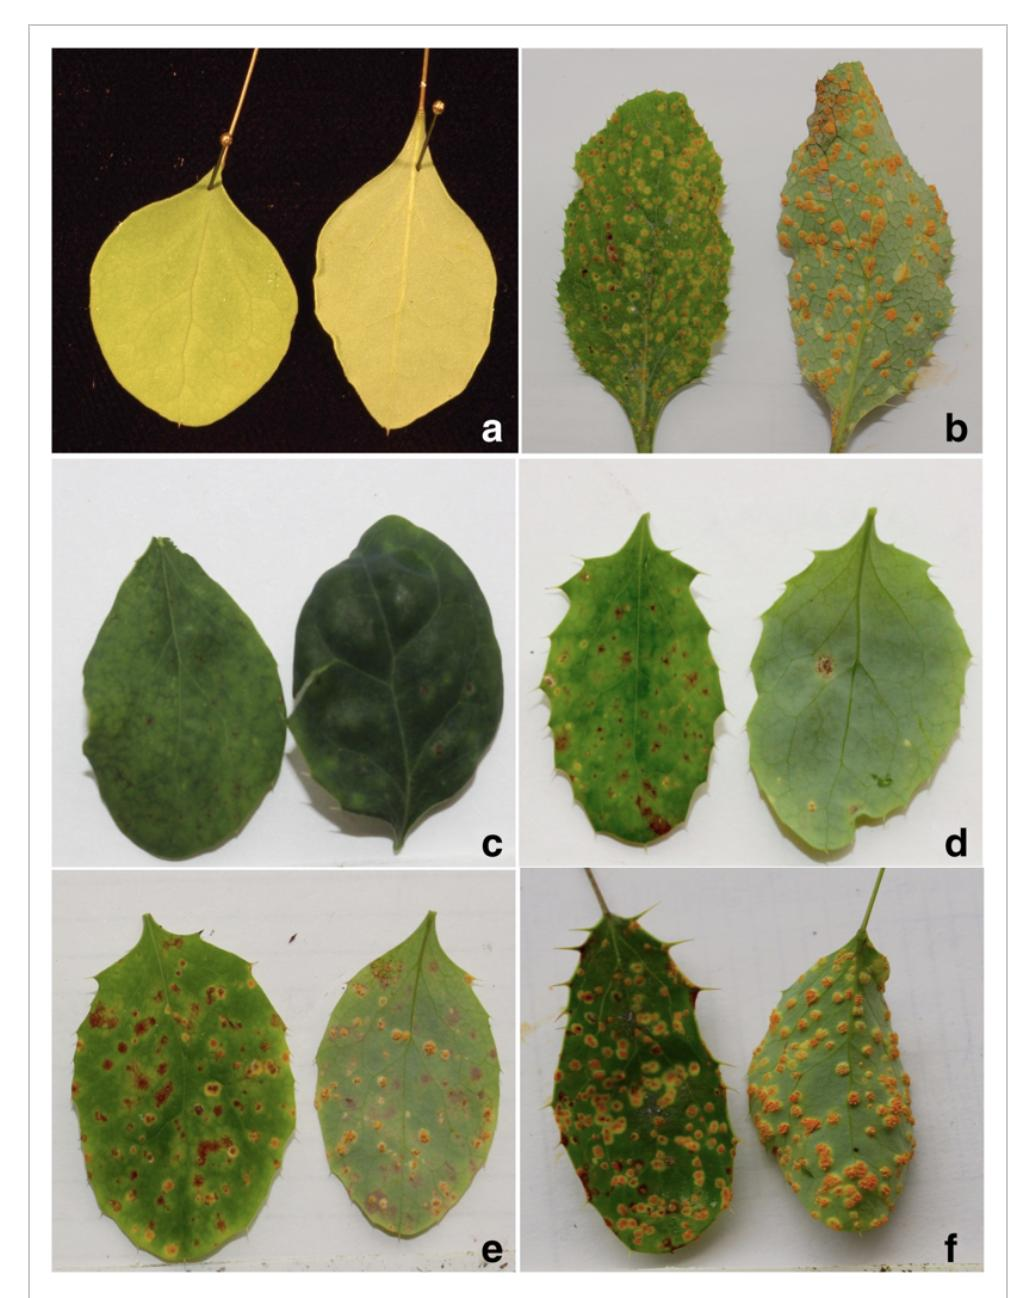
\includegraphics[width=0.28\linewidth]{../images/non-host-resistance-stem-rust} \caption{Representative disease response of the two mapping population parents and their $F_1$ progeny. (a) Resistant reaction of \textit{B. thunbergii} accession 'BtUCONN1' showing no visual symptoms; (b) Susceptible reaction of \textit{B. vulgaris} accession 'Wagon Hill', showing dense pycnia on the upper leaf surface and prolific, well-developed aecia on the lower surface; (c) Resistant reaction (score 1 on the four-point scale) of \textit{B. x ottawensis} progeny 'WH15-039', showing sparse flecking; (d) Moderate resistant reaction (score 2) of \textit{B. x ottawawensis} progeny 'WH15-063', showing evident necrotic lesions and some pycnia formation; (e) Moderate susceptible reaction (score 3) of \textit{B. x ottawensis} progeny 'WH15-128', showing well-developed pycnia and aecia, alogside sparse necrotic lesions; and (f) Susceptible reaction (score 4) of \textit{B x ottawensis} progeny 'WH15-149', showing well-developed pycnia and aecia and no evident necrosis. All photos were taken 14 days post-inoculation.}\label{fig:non-host-resistance}
\end{figure}

\end{columns}

\footnotesize Note: Refer to Bartaula et al. (2019) for details on
mapping of non-host resistance to stem rust.
\end{frame}

\begin{frame}{}
\protect\hypertarget{section-4}{}
\footnotesize

Weeds harboring various pathogenic fungi. Different symptoms observed on
the sampled symptomatic weed species. Symptoms were identified in
different groups as follows: black necrosis (blN), brown felting (brF),
brown necrosis (brN), chlorosis (C), orange pustule (oP), pink necrosis
(pN), powdery mildew (pM), rust (R), and white pustule (wP).

\begin{columns}\column{0.5\textwidth}

\begin{center}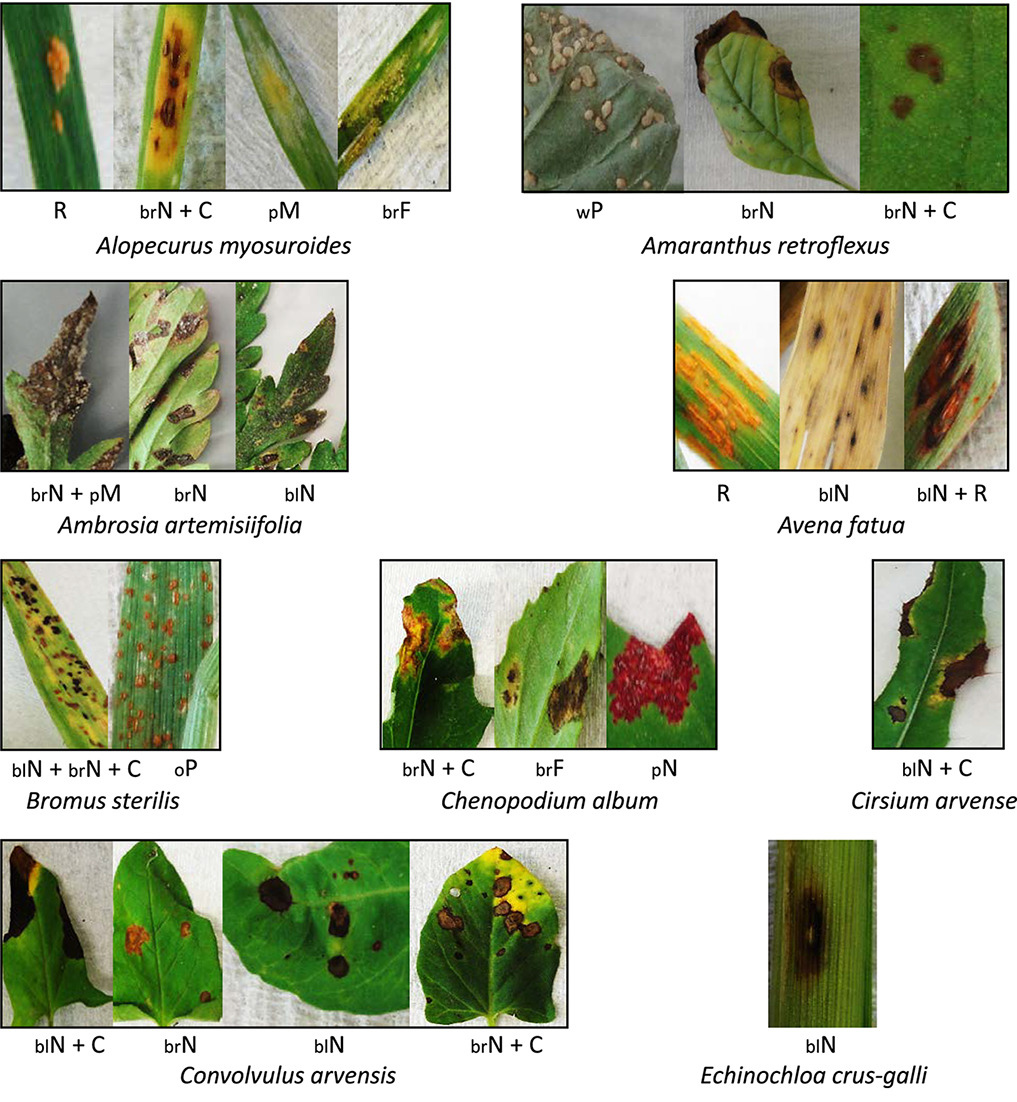
\includegraphics[width=0.54\linewidth]{../images/host-species1} \end{center}

\column{0.5\textwidth}

\begin{center}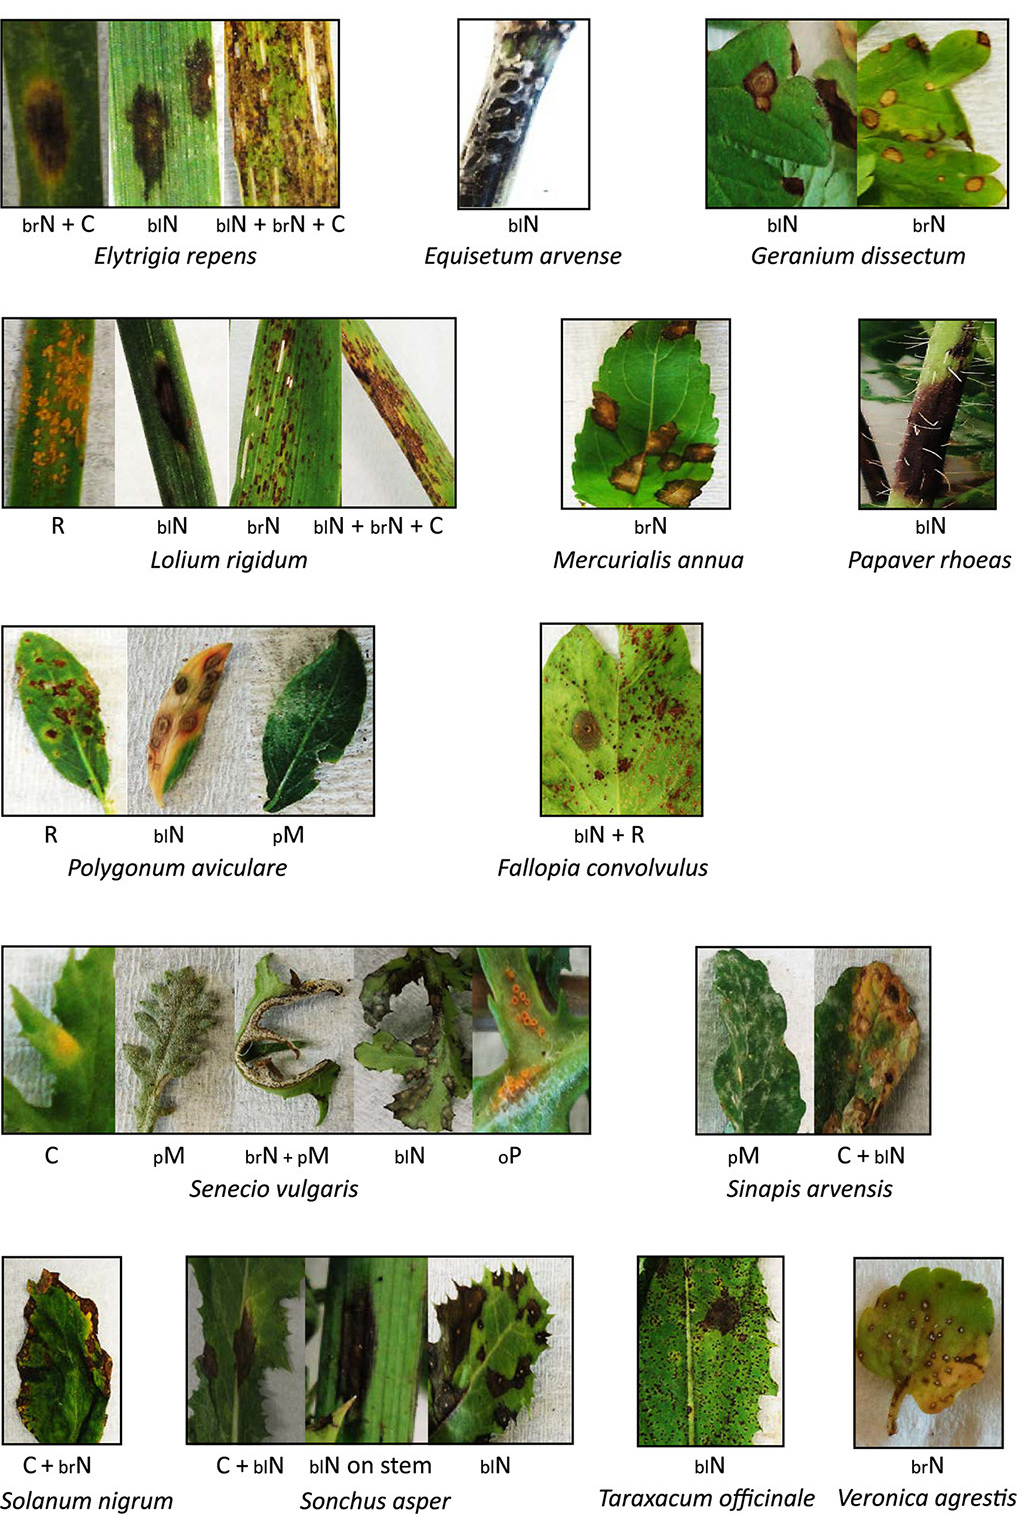
\includegraphics[width=0.54\linewidth]{../images/host-species2} \end{center}

\end{columns}
\end{frame}

\hypertarget{application-of-non-durable-resistance}{%
\section{Application of non-Durable
Resistance}\label{application-of-non-durable-resistance}}

\hypertarget{gene-pyrimiding}{%
\section{Gene Pyrimiding}\label{gene-pyrimiding}}

\begin{frame}{Gene Pyrimiding}
\small

\begin{itemize}
\tightlist
\item
  If all genes cannot be fixed in a single step of selection, it is
  necessary to cross again selected individuals with incomplete, but
  complementary, sets of homozygous loci.
\item
  Pyramiding of \(R\) genes in a variety provides opportunity for
  simulataneous expression of more than one gene in a variety so that
  breakdown of host resistance is delayed.
\item
  \(R\) gene pyramids generally result from introgression of a new \(R\)
  gene into an adapted variety with an existing complement of `defeated'
  \(R\) genes -- avoids the issue of agronomic performance of the
  pyramid (recipient) variety.
\item
  In theory pyramiding several `undefeated' \(R\) genes should provide
  more durable resistance since mutational events at several \(Avr\)
  loci would be required to produce a new virulent pathotype.
\end{itemize}
\end{frame}

\begin{frame}{}
\protect\hypertarget{section-5}{}
\small

\begin{itemize}
\tightlist
\item
  Gene pyramiding is nearly impossible through conventional means due to
  dominance and epistasis effects of genes governing disease resistance
  and linkage with undesirable traits that is difficult to break.
\item
  MAS for molecular markers linked to \(R\) genes or for the \(R\) genes
  themselves, enables pyramiding of several effective \(R\) genes.
\item
  Even in genomes with clustered \(R\) genes, MAS may be be used select
  for rare recombinants containing loci in coupling to create new \(R\)
  gene combinations for which the matching virulence may not readily
  evolve.
\end{itemize}

(\footnotesize Refer to Ye, Smith, et al. (2010) (or Volume 33, Plant
Breeding Reviews) for extensive discussion)
\end{frame}

\begin{frame}{}
\protect\hypertarget{section-6}{}
\begin{figure}
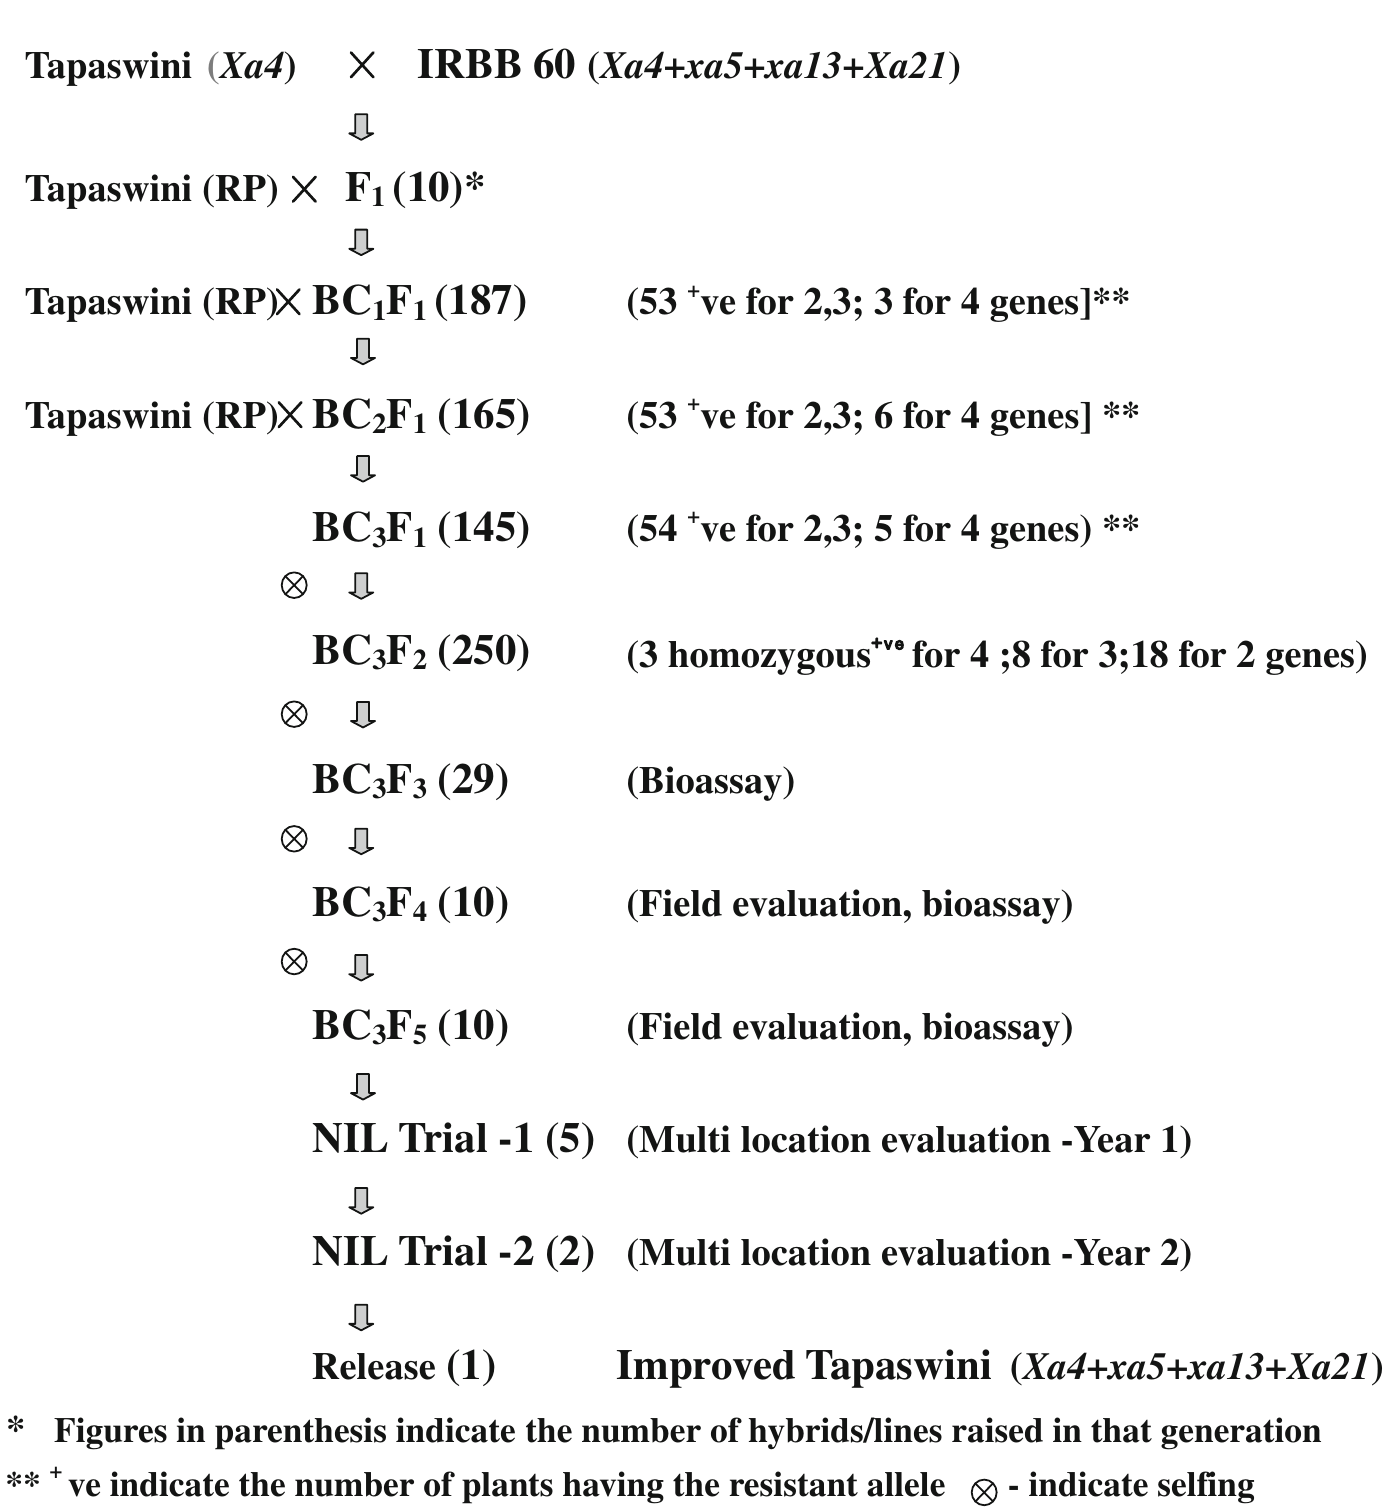
\includegraphics[width=0.38\linewidth]{../images/gene_pyramiding_rice_blast} \caption{Tapaswini (rice variety popular in eastern India) has high and stable yield but is susceptible to bacterial blight. Study introgressed 4 resistance genes -- $Xa4$, $xa5$, $xa13$ and $Xa21$ -- from a donor IRBB 60, a gene pyramid developed at IRRI, Philippines, with Tapaswini as recurrent parent. Conventional BC was followed upto BC3 and around 150 plants/lines were genotyped at each generation for the presence of the target genes and only positive plants having the resistance alleles were advanced to the next generation. Foreground selection continued till BC3F3 to identify pure homozygous lines for all four target genes. Selection based on morphological and grain quality traits was practiced from BC3F2 onwards for recovery of recurrent parent characteristics. The latter was assisted by selection with SSR marker}\label{fig:gene-pyramiding-rice-blast}
\end{figure}
\end{frame}

\hypertarget{multilines-cultivar-mixtures}{%
\section{Multilines, Cultivar
Mixtures}\label{multilines-cultivar-mixtures}}

\begin{frame}{Multilines, Cultivar Mixtures}
\begin{itemize}
\tightlist
\item
  Wild plants appear to use heterogeneity for R genes as a strategy for
  avoiding disease epidemics.
\item
  Growing crops heterogeneous for their R gene complement inflicts
  disruptive selection upon the pathogen population reducing the
  selection pressure against any one avirulence allele or combination of
  avirulence alleles -- idea of multilines or variety mixtures.
\item
  Multilines and mixtures can be distinguished by the relationship
  between their components.

  \begin{itemize}
  \tightlist
  \item
    In multilines, the components are usually closely related
  \item
    In mixtures, the components can be unrelated or distantly related.
  \item
    Variety mixtures are more haphazardly composed than multilines and
    are often considered as a deployment strategy rather than a breeding
    strategy
  \end{itemize}
\end{itemize}
\end{frame}

\begin{frame}{}
\protect\hypertarget{section-7}{}
\begin{itemize}
\tightlist
\item
  There is convincing evidence that crop heterogeneity for R gene
  complement reduces the incidence of disease in modern agricultural
  systems.
\item
  A major concern in using multilines/mixtures has been whether they
  would select for complex races.

  \begin{itemize}
  \tightlist
  \item
    Studies in \textit{E. graminis} in barley have suggested there is
    little unidirectional selection for complex races and their
    evolution will be slow.
  \item
    Any loss of resistance in the mixture/multiline is more likely to be
    due to an increase in frequency of a simpler pathotype with matching
    virulence to one component.
  \end{itemize}
\end{itemize}

(Refer to Chapter 4 of Newton et al. (1997) and Chapter 17 of Reddy
(2017).)
\end{frame}

\begin{frame}{}
\protect\hypertarget{section-8}{}
\small

\begin{itemize}
\tightlist
\item
  Advantage of multilines over mixtures is due to their greater
  agronomic uniformity. However, they take time and effort to breed and
  it can be difficult to respond to changes in market requirements or in
  the frequency of virulence alleles in the pathogen population.
\item
  Mixtures were proposed as a pragmatic alternative to multilines.

  \begin{itemize}
  \footnotesize
  \item It is possible to respond relatively rapidly to changes in the frequency of virulence alleles within a pathogen population or the relative importance of different pathogens by changing the mix of varieties.
  \item However, because breeders have continually introgressed new R genes into adapted varieties thereby maintaining defeated $R$ genes in the crop, it can be difficult to find components with sufficient $R$ gene diversity.
  \item Greater 'background' heterogeneity can buffer mixtures against abiotic stresses providing greater yield stability.
  \item An alternative would be the use of transformation to produce 'mix and match' multilines by transforming elite cultivars with different transgenes giving isogenic (uniform) components differing only in their $R$ gene complement
  \item As with pyramiding transgenes, the transgenic multiline approach requires a collection of cloned $R$ genes.
  \end{itemize}
\end{itemize}
\end{frame}

\hypertarget{integrated-control}{%
\section{Integrated Control}\label{integrated-control}}

\begin{frame}{}
\protect\hypertarget{section-9}{}
\begin{itemize}
\tightlist
\item
  Allelopathy is a naturally occuring ecological phenomenon of
  interference among organisms.

  \begin{itemize}
  \tightlist
  \item
    a pragmatic approach to resolving multiple issues, including pest
    management, stress management and growth enhancement
  \item
    resolves problem of resistance development, soil and environment
    pollution caused by non-judicious use of synthetic pesticides
  \item
    employed through crop rotations, crop cover, intercropping,
    mulching, incorporation of crop residues, and application of
    botanical extracts
  \item
    strategy could be used in multiple conjunctions
  \end{itemize}
\item
  Allelopathy is the result of chemicals released (allelochemicals),
  mostly secondary metabolites produced by plants. \bdescription

  \item[Allelochemicals]

  alkaloids, amino acids, brassinosteroids, carbohydrates, flavonoids,
  glucosinolates, hydroxamic acids, jasmonates, momilactone, phenolics,
  salicylates, and terpenoids \edescription
\end{itemize}
\end{frame}

\begin{frame}{Weed and host crop management}
\protect\hypertarget{weed-and-host-crop-management}{}
\small

\begin{itemize}
\tightlist
\item
  Allelopathic species suppress weeds when employed in the field
  following crop rotation, or as cover/smother crops, intercrops, crop
  residues.
\item
  Soil application of essential oils from (possibly) intercropped plants
  such as \emph{Mentha} spp., \emph{Satureja montana} and those of genus
  \emph{Ocimum} can replace commonly used methyl bromid for soil
  fumigation against soil-borne pathogens
\item
  Aggressive competitors crops like sweet potato ( \emph{Ipomoea
  batatas}) can be utilized for successful management of noxious weeds
  and parasitic plants such as strigas ( \emph{Striga hermonthica} and
  \emph{Striga asiatica})
\item
  Intercropping of maize with leguminous plants such as greenleaf
  Desmodium is employed for effective management of \emph{S. hermothica}

  \begin{itemize}
  \tightlist
  \item
    C-glycosylflavonoid called isoschaftoside released by Desmodium is
    the allelochemical responsible for suppression of Striga
  \end{itemize}
\item
  In rice-wheat system, integration of smothering allelopathic crops,
  such as maize, perl millet or sorghum after harvesting wheat and
  before rice transplantation offers effective weed suppression for
  upcoming rice crop.
\end{itemize}
\end{frame}

\begin{frame}{}
\protect\hypertarget{section-10}{}
\small

\begin{itemize}
\tightlist
\item
  Wheat rotated with Egyptian clover or oat provides natural weed
  control.
\item
  Cover crops suppress weeds through chemical allelopathy when used as
  green manure by inhibiting weed seed germination.

  \begin{itemize}
  \tightlist
  \item
    Barnyard grass ( \emph{Echinochloa crus-galli}) population was
    substantially reduced in maize by the use of bean as legume cover
    crop.
  \end{itemize}
\item
  Noxious paddy weeds such as Barnyard grass, flat sedge( \emph{Cyperus
  difformis}), jungle rice ( \emph{Echinochloa colonum}) can be
  suppressed by more than 70\% through application of allelopathic plant
  mulches.
\item
  Water extract of sorghum plant as a natural herbicide is illustrated
  in wheat, cotton and sunflower, which suppresses weed biomass and
  density (\textasciitilde45\%) of \emph{C. album}, \emph{Fumaria
  indica}, \emph{P. minor} and \emph{Rumex dentatus}, with simultaneous
  increase in grain yield.
\end{itemize}
\end{frame}

\begin{frame}{Insect pest management}
\protect\hypertarget{insect-pest-management}{}
\begin{itemize}
\tightlist
\item
  Chemicals of plant origin such as azadirachtin, nimbin and salanin in
  neem reduce/inhibit growth of insects like cicadellid and white fly
  (Bemisia tabaci)
\item
  Neem oil serves anti-feedant action against strawberry aphids
\item
  Flower thrips ( \emph{Taeniothrips sjostedti}) and pod borer (
  \emph{Heliothis armigera}) in common beans are effectively controlled
  by plant extracts of tomato.
\item
  Allelochemicals from weeds like chick weed ( \emph{Ageratum
  conyzoides}), great ragweed ( \emph{Ambrosia trifida}), and Spanish
  flag (Lantana camara) were not only inhibitory to insects such as
  cowpea weevil ( \emph{Callosobruchus maculatus})
\item
  Stored grain insects have been known to be affected by:

  \begin{itemize}
  \tightlist
  \item
    \emph{Sitophilus oryzae}: Bakaino, habulas ( \emph{Myrtus
    communis}), lemon grass ( \emph{Cymbopogon citratus}) and mint
  \item
    \emph{Callosobruchus chinensis}: \emph{Cannabis sativa}, black
    pepper and garlic
  \item
    \emph{Corcyra cephalonica}: Red chillies and tea
  \end{itemize}
\end{itemize}
\end{frame}

\begin{frame}{Disease management}
\protect\hypertarget{disease-management}{}
\small

\begin{itemize}
\tightlist
\item
  Plant extracts like canola, different cereals, lentil, and sweet
  clover at low concentrations was very effective in suppressing the
  fungus \emph{Sclerotinia sclerotiorum} in beans
\item
  The allelochemicals produced by rice (momilactone A and momilactone B)
  exhibited antibacterial, antifungal, antioxidant and anticancer
  activities in vitro while the flavones and cyclohexenones had effect
  of suppressed spore formation of \textit{P. oryzae} and
  \textit{Rhizoctonia solanacearum} (Bacterial wilt agent).
\item
  Wheat rust is controlled by leaf extract of jimson weed ( \emph{Datura
  stramonium})
\item
  50\% growth reduction of Fusarium solani was caused by leaf water
  extracts of eucalyptus, neem, and tulsi.
\item
  Intercropping of tomato with Chinese chive ( \emph{Allium tuberosum})
  suppressed bacterial wilt.
\item
  Intercropping of tomato with marigold ( \emph{Tagetes erecta})
  controlled tomato early blight disease caused by \emph{Alternaria} by
  more than 90\% through the release of certain volatile allelochemicals
  exuded from the aerial parts.
\end{itemize}
\end{frame}

\begin{frame}{Nematode management}
\protect\hypertarget{nematode-management}{}
\begin{itemize}
\tightlist
\item
  Soil application of allelochemicals from neem leaves or neem cakes
  reduces the development of root-knot nematodes ( \emph{Meloidogyne
  javanica}).
\item
  Soil incorporation of \emph{Brassica} spp. releases sulfur compounds
  (glucosinolates), which are converted into isothiocyanates which
  inturn serve as natural nematicidal fumigants.
\end{itemize}
\end{frame}

\hypertarget{bibliography}{%
\section{Bibliography}\label{bibliography}}

\begin{frame}[allowframebreaks]{References}
\protect\hypertarget{references}{}
\footnotesize

\hypertarget{refs}{}
\begin{CSLReferences}{1}{0}
\leavevmode\vadjust pre{\hypertarget{ref-bartaula2019mapping}{}}%
Bartaula, Radhika, Arthur TO Melo, Sarah Kingan, Yue Jin, and Iago Hale.
2019. {``Mapping Non-Host Resistance to the Stem Rust Pathogen in an
Interspecific Barberry Hybrid.''} \emph{BMC Plant Biology} 19 (1):
1--17.

\leavevmode\vadjust pre{\hypertarget{ref-leach2001pathogen}{}}%
Leach, Jan E, Casiana M Vera Cruz, Jianfa Bai, and Hei Leung. 2001.
{``Pathogen Fitness Penalty as a Predictor of Durability of Disease
Resistance Genes.''} \emph{Annual Review of Phytopathology} 39 (1):
187--224.

\leavevmode\vadjust pre{\hypertarget{ref-newton1997cultivar}{}}%
Newton, AC et al. 1997. {``Cultivar Mixtures in Intensive
Agriculture.''} \emph{The Gene-for-Gene Relationship in Plant-Parasite
Interactions.}, 65--80.

\leavevmode\vadjust pre{\hypertarget{ref-reddy2017agro}{}}%
Reddy, P Parvatha. 2017. \emph{Agro-Ecological Approaches to Pest
Management for Sustainable Agriculture}. Springer.

\leavevmode\vadjust pre{\hypertarget{ref-ye2010marker}{}}%
Ye, Guoyou, Kevin F Smith, et al. 2010. {``Marker-Assisted Gene
Pyramiding in Cultivar Development.''} \emph{Molecular Plant Breeding:
Principle, Method and Application}, 321--42.

\end{CSLReferences}
\end{frame}




\end{document}
